\chapter{Opis teoretyczny wybranych algorytmów}
\label{cha:opis_teoretyczny_wybranych_algorytmow}
%%TODO metody segm ob pierwsz. i tej terminologii bym się trzymał....

\section{Proste metody segmentacji obiektów pierwszoplanowych}
\label{sec:proste_metody}

W tym rozdziale przedstawiono kilka prostych obliczeniowo metod segmentacji tła. Oczywiście, uzyskane z ich wykorzystaniem wyniki, znacząco odbiegają, od tego co oferują zaawansowane algorytmy. Szczególnie podczas testów w bardziej wymagającym środowisku, na przykład w przypadku drgań kamery lub z obecnością dynamicznego tła. %TODO przykład w nawiasie - przyklad czego?
Mimo to, często znajdują zastosowanie w mniej wymagających systemach, właśnie ze względu na swoją prostotę i w rezultacie niską złożoność obliczeniową.
%%TODO i idącą za tym niską złożonością obliczeniową.

Pierwszym omawianym podejściem jest \textbf{metoda naiwna}. 
W tym algorytmie, przyjmujemy założenie, że pierwsza ramka jest modelem referencyjnym tła i nie zawiera żadnych obiektów pierwszoplanowych. 
Proces segmentacji tła polega na obliczeniu różnicy między aktualną ramką, a zapisanym modelem. 
Jeżeli dla konkretnego piksela otrzymana różnica jest większa od przyjętej wartości progowej zostaje on uznany za element pierwszego planu. 
Przedstawiony algorytm oczywiście nadaje się jedynie do prostej segmentacji i nie zapewnia akceptowalnych rezultatów podczas pracy w bardziej wymagającym środowisku.

Koleją prostym algorytmem jest technika \textbf{odejmowania ramek}, w tym przypadku również wykonywane jest odejmowanie modelu referencyjnego i aktualnej ramki. 
Jako model referencyjny wykorzystywana jest poprzednia ramka obrazu. 
Metoda ta nadaje się niestety jedynie do detekcji obiektów ruchomych. 
W niniejszej pracy algorytm ten został również wykorzystany jako element mechanizmu detekcji tzw. ,,duchów'', całość została szczegółowo przedstawiona w rozdziale \ref{subsec:pbas_duchy}.

Ostatnia spośród prostych metod to tzw. \textbf{adaptacyjne odejmowanie tła}, technika ta jest w pewnym stopniu rozszerzeniem opisanej powyżej metody naiwnej. 
W tym przypadku także wykonywane jest odejmowanie modelu tła i aktualnej ramki obrazu, a następnie dokonywanie klasyfikacji poprzez progowanie. 
Nieco bardziej złożona jest procedura aktualizacji modelu tła. 
Jest ona wykonywana po każdej ramce obrazu i została zapisana równaniem (\ref{equ:adaptive_bg_sub}).

	\begin{equation}
	    B(t) = \alpha I(t) + (1 - \alpha)B(t-1) 
	\label{equ:adaptive_bg_sub}
	\end{equation}	
	
\noindent gdzie:
\begin{eqwhere}[2cm]
 \item[$B(t)$] model tła w chwili $t$
 \item[$I(t)$] obraz wejściowy w chwili $t$
 \item[$\alpha$] parametr z zakresu od 0 do 1\\
\end{eqwhere}

%%TODO równianie na segmentację. Komentarz, że to może być w różnych przestrzeniach barw.
Warto zaznaczyć, że wszystkie trzy, wymienione algorytmy mogą przetwarzać obraz w różnych przestrzeniach barw, najpopularniejsza jest oczywiście standardowa przestrzeń kolorów \textit{RGB}. W tym przypadku do obliczenia różnicy, koniecznej do segmentacji, wykorzystuje się metrykę euklidesową. Ostateczny wzór na klasyfikację piksela przedstawiono równaniem \ref{equ:simple_seg_rgb}. Druga odmianą może być obraz w skali szarości, w takiej sytuacji obliczenia są uproszczone, gdyż konieczne jest wyznaczenie jedynie modułu z różnicy.

    \begin{equation}
        F(x,y) = 
		\begin{dcases}
    		1, & \text{gdy } \sum_{C \in \{R,G,B\}} | I(x,y,C) - B(x,y,C) | > T \\
    		0, & \text{w pozostałych przypadkach} 
		\end{dcases}        
    \label{equ:simple_seg_rgb}
    \end{equation}     

\noindent gdzie:
\begin{eqwhere}[2.5cm]
 \item[$F(x,y)$] wyjściowa maska binarna piksela o współrzędnych $x$, $y$
 \item[$I(x,y,C)$] pojedyncza składowa piksela wejściowego o współrzędnych $x$, $y$
 \item[$B(x,y,C)$] pojedyncza składowa piksela z modelu tła o współrzędnych $x$, $y$
 \item[$T$] próg klasyfikacji (dla przestrzeni \textit{RGB} domyślnie $50$)\\
\end{eqwhere}

\section{Visual Background Extractor}
\label{sec:vibe_teoria}
%%TODO proszę podać referencję do oryginalnej wersji artykułu - zotała podana w drugim akapicie

Algorytm nazywany w skrócie \textit{ViBE} (\textit{Visual Background Extractor}), jak zostało wspomniane w rozdziale \ref{sec:model_poprzednie_ramki}, jest metodą bazującą na modelu opartym o wartości pikseli obserwowane w poprzednich ramkach obrazu. 
%%TODO raczej w wartości pikseli obserwowane w poprzednich ramkach ?
Warto ponownie podkreślić, że zapamiętane wartości pikseli z poprzednich ramek obrazu to jedyna informacje wykorzystywane przez ten algorytm. Podobnie jak większość innych metod, \textit{ViBE} może zostać dostosowane do pracy z~różnymi przestrzeniami barw (np. \textit{RGB}, skala szarości, \textit{CIELab}).

Opisana w niniejszej pracy wersja algorytmu została przedstawiona w publikacji \cite{kryjak_14_vibe}. 
Standardową wersję metody dostosowano do pracy z poruszającą się kamerą. 
Realizowane jest to, poprzez mechanizm przesunięcia modelu tła. 
W celu wyznaczenia wektora przesunięcia wykorzystywane jest obliczenie rzadkiego przepływu optycznego, dokładne szczegóły takiego rozwiązania, zostały zaprezentowane w~podrozdziale \ref{subsec:vibe_of}.

\subsection{Opis algorytmu}
\label{subsec:vibe_opis}

Model tła zdefiniowany jest osobno dla każdego piksela i składa się z $N$ próbek (tj. wartości pikseli). 
Proces inicjalizacji jest bardzo prosty i trwa tylko jedną ramkę obrazu. 
Każda z $N$ próbek inicjalizowana jest losowo, wartością odpowiadającego jej piksela lub któregoś z jego sąsiadów. 
W tym przypadku przez sąsiedztwo rozumiemy przestrzenny kontekst $3x3$, czyli jedynie najbliższe otaczające piksele. 

Zdefiniujmy wartość piksela (o współrzędnych $x$, $y$) w wybranej przestrzeni barw jako $\upsilon(x,y)$, z~kolei i-tą próbkę z modelu tła oznaczmy jako $\upsilon_i$. 
Model tła dla konkretnego piksela, możemy wtedy zapisać za pomocą wzoru (\ref{equ:vibe_model}).

	\begin{equation}
		M(x,y)= \left\{ \upsilon_1, \upsilon_2, \dotsc, \upsilon_N \right\}
	\label{equ:vibe_model}	
	\end{equation}
	
W celu przeprowadzenia klasyfikacji nowego piksela i przypisania mu etykiety obiektu pierwszoplanowego lub tła, należy zdefiniować okrąg $S(\upsilon(x,y))$ o środku w punkcie $\upsilon(x,y)$ i promieniu $R$. 
Promień ten jest wartością stałą, identyczną dla każdego modelu. 
Piksel uznawany jest za pierwszoplanowy jeżeli przynajmniej $\#_{min}$ próbek z modelu tła zawiera się wewnątrz takiego okręgu. 
Oznaczmy przez $F$~maskę reprezentującą obiekty pierwszoplanowe ($1$ -- piksel pierwszoplanowy, $0$ -- tło), wówczas opisany warunek przedstawia równanie (\ref{equ:vibe_test}).

	\begin{equation}
	    F(x,y) = 
		\begin{dcases}
    		1, & \text{gdy } \sum_{k=0}^{N} \{ d(\upsilon(x,y), \upsilon_k(x,y)) < R \} < \#_{min} \\
    		0, & \text{w pozostałych przypadkach} 
		\end{dcases}
	\label{equ:vibe_test}	
	\end{equation}
\noindent gdzie $d$ to funkcja odległości pomiędzy próbką z modelu tła, a aktualnym pikselem.

Sposób obliczania odległości zależy od przyjętej przestrzeni barw. 
Można wykorzystać obraz w skali szarości, standardową przestrzeń \textit{RGB} lub \textit{CIELab}. 
W przypadku dwóch pierwszych wykorzystywana jest prosta metryka miejska, czyli inaczej suma modułów różnicy każdej składowej. 
Alternatywnym rozwiązaniem, aczkolwiek bardziej złożonym obliczeniowo jest metryka euklidesowa. 
Autorzy artykułów \cite{kryjak_14_vibe, kryjak_13_vibe} zdecydowali się na wykorzystanie przestrzeni \textit{CIELab}. Algorytm konwersji z przestrzeni \textit{RGB} został opisany w rozdziale \ref{subsec:vibe_cielab}, natomiast odległość między próbkami jest przedstawiona równaniem~(\ref{equ:vibe_cielab_test}).

	\begin{equation}
	    d_{CIELab} = \alpha \cdot |L_I - L_B| + \beta \cdot (| a_I - a_B | + | b_I - b_B |)
	\label{equ:vibe_cielab_test}
	\end{equation}
Gdzie:
\begin{eqwhere}[2.6cm]
	\item[$L_I,\, a_I,\, b_I$] składowe piksela wejściowego
	\item[$L_B,\, a_B,\, b_B$] składowe zapisane w modelu tła
	\item[$\alpha,\, \beta$] wagi wynoszące odpowiednio \num{1} i \num{1.5}
\end{eqwhere}

%%TODO komentarz o tym, dlaczego rozbicie jest istotne
\noindent Składowa jasności \textit{L} ma mniejsze znaczenie, w kontekście rozróżniania obiektów, od składowych chrominancji \textit{a} i \textit{b}. W związku z tym, eksperymentalnie zastosowano w jej przypadku minimalnie niższą wagę.  

W omawianej metodzie wykorzystano konserwatywną politykę aktualizowania modelu tła -- szczegółowe różnice pomiędzy podejściem liberalnym a konserwatywnym zaprezentowano w rozdziale \ref{sec:model_tla_aktualizacja}. 
Aktualizacji podlegają zatem jedynie modele reprezentujące obszar zaklasyfikowany jako tło.
W trakcie aktualizacji, wprowadzony został element losowy. Mianowicie dla każdego modelu tła podejmowana jest decyzja (w sposób całkowicie losowy), czy należy dokonywać aktualizacji. 
Przyjęto, że prawdopodobieństwo wykonania uaktualnienia jest stałe i reprezentowane przez parametr $T$. 

Sam proces jest bardzo prosty, kiedy już dany model zostanie zakwalifikowany do zaktualizowania wybierana jest losowa próbka i jej wartość zostaje nadpisana przez aktualną wartość piksela $\upsilon(x,y)$. 
Dodatkowo wybierany jest losowo jeden model z najbliższego sąsiedztwa (kontekst przestrzenny o rozmiarze $3x3$) aktualnie analizowanego piksela i w nim także jedna losowo wybrana próbka zostaje nadpisana wartością $\upsilon(x,y)$. Takie działanie ma na celu, częściową eliminację negatywnych skutków konserwatywnego podejścia do aktualizacji modelu. 
%%TODO napisać po co to

Warto podkreślić, że algorytm \textit{ViBE} w omówionej tutaj, podstawowej wersji wymaga bardzo niedużej liczby parametrów. 
Należy zdefiniować jedynie liczbę próbek $N$ zapisanych w każdym modelu, promień $R$ okręgu wykorzystywanego w teście dopasowania, wymaganą minimalną liczbę próbek $\#_{min}$, leżącą wewnątrz wspomnianego okręgu oraz prawdopodobieństwo wykonania aktualizacji $T$.


\subsection{Konwersja RGB -- CIELab}
\label{subsec:vibe_cielab}

Konwersja z przestrzeni \textit{RGB} do \textit{CIELab} jest stosunkowo złożona pod względem matematycznym, jednak jak zauważono, między innymi w publikacjach \cite{kryjak_13_vibe, kryjak_14_vibe}, wykorzystanie tej przestrzeni kolorów daje znacznie dokładniejsze wyniki segmentacji. 
W związku z powyższym, omawiany algorytm w finalnej implementacji sprzętowej będzie zrealizowany z wykorzystaniem właśnie tej przestrzeni barw. 

Proces konwersji składa się z dwóch etapów. 
Pierwszym krokiem jest przekształcenie składowych \textit{RGB} do przestrzeni \textit{CIE XYZ}, jest to operacja liniowa zapisana równaniem (\ref{equ:vibe_rgb_xyz}).

	\begin{equation}
		\begin{bmatrix}
			X \\
			Y \\
			Z \\
		\end{bmatrix}
		=
		\begin{bmatrix}
			0.41245 & 0.35758 & 0.18042 \\
			0.21267 & 0.71516 & 0.07217 \\
			0.01933 & 0.11919 & 0.95923 \\
		\end{bmatrix}
		\begin{bmatrix}
			R \\
			G \\
			B \\
		\end{bmatrix}
	\label{equ:vibe_rgb_xyz}	
	\end{equation}	 

Następna operacja to przekształcenie z właśnie otrzymanej przestrzeni \textit{CIE XYZ} do docelowej \textit{CIELab}. 
W tym celu wykorzystywana jest funkcja $f(t)$ opisana równaniem (\ref{equ:vibe_f_t}). 
Ostatecznie wyznaczenie składowej jasności -- $L$ i dwóch składowych chrominacji -- $a$ i $b$ przedstawia wzór \ref{equ:vibe_xyz_cielab}. Wykorzystane współczynniki wynoszą odpowiednio $X_n = 0.950465$, $Y_n = 1$, $Z_n = 1.088754$

	\begin{equation}
	    f(t) = 
		\begin{dcases}
    		t^{-3}, & \text{dla } t > \left( \frac{6}{29} \right)^3 \\
    		\frac{1}{3} \left( \frac{29}{6} \right)^2 t + \frac{4}{29}, 
    		& \text{w przeciwnym razie} 
		\end{dcases}
	\label{equ:vibe_f_t}	
	\end{equation}


	\begin{equation}
		\begin{bmatrix}
			L \\
			a \\
			b \\
		\end{bmatrix}
		=
		\begin{bmatrix}
			116 f(\frac{Y}{Y_n}) - 16 \\
			500 \left[ f(\frac{X}{X_n}) - f(\frac{Y}{Y_n}) \right]\\
			200 \left[ f(\frac{Y}{Y_n}) - f(\frac{Z}{Z_n}) \right] \\
		\end{bmatrix}
	\label{equ:vibe_xyz_cielab}
	\end{equation}

Z równań (\ref{equ:vibe_f_t}) i (\ref{equ:vibe_xyz_cielab}) można wywnioskować, że składowa $L$ przyjmuje wartości z zakresu $0$ -- $100$, natomiast składowe chrominacji $a$ i $b$ mieszczą się w przedziale od $-128$ do $127$. 
Warto zwrócić uwagę, że ze względu na skomplikowane obliczenia matematyczne (funkcja $f(t)$), implementacja sprzętowa takiej konwersji jest bardzo utrudniona, problem ten oraz jego rozwiązanie zostało szczegółowo opisane w rozdziale \ref{sec:fpga_vibe}.

\subsection{Obsługa ruchomej kamery}
\label{subsec:vibe_ruchoma_kamera}

Kompletny algorytm segmentacji obiektów pierwszoplanowych musi między innymi poprawnie funkcjonować w przypadku lekkich drgań lub delikatnego przemieszczania się kamery. Rozwiązanie zapewniające taką funkcjonalność zostało zaprezentowanie między innymi w publikacji \cite{kryjak_14_vibe} i polega na oszacowaniu przesunięcia kamery na podstawie badania przepływu optycznego. %%TODO brak cytowania !

Oznaczmy oszacowane przesunięcie kamery pomiędzy dwiema kolejnymi klatkami jako wektor $[dx,dy]$. 
Metoda wyznaczania tego przesunięcia została przedstawiona w rozdziale \ref{subsec:vibe_of}. 
W~celu kompensacji ruchu kamery stosuje się przesunięcie modelu tła zgodnie z równaniem (\ref{equ:vibe_bg_shift}).

	\begin{equation}
	M_t(x,y) = M_{t-1}(x+dx,y+dy)
	\label{equ:vibe_bg_shift}
	\end{equation}
gdzie przez $M_t(x,y)$ rozumiemy model tła dla piksela o współrzędnych $x$, $y$ w chwili $t$.


Jak łatwo zauważyć, po takiej operacji część modeli tła, związana ze skrajnymi pikselami została usunięta i wymaga ponownej inicjalizacji. W tym przypadku, zamiast losowego inicjalizowania, opartego na wartości sąsiednich pikseli, do wszystkich próbek w danym modelu przypisana zostaje aktualna wartość piksela. Takie działanie jest konieczne, ponieważ nie ma możliwości wyznaczenie sąsiedztwa dla skrajnych pikseli.
%%TODO gdyż zwykle jest to jedna skrajna linia...

\subsection{Wyznaczanie rzadkiego przepływu optycznego}
\label{subsec:vibe_of}

Wspomniany w poprzednim podrozdziale wektor przesunięcia, może zostać oszacowany poprzez wyznaczenie przepływu optycznego. 
W przypadku opisywanej metody, należy przyjąć założenie, że przesunięcie jest identyczne na obszarze całego obrazu. 
Obliczanie przepływu nie jest wykonywane na całej ramce obrazu, a jedynie na reprezentatywnej grupie pikseli (tzw. rzadki przepływ optyczny). 
Wybierane są takie fragmenty, na których najprościej śledzić przesunięcie, w tym przypadku zdecydowano się na analizę pikseli reprezentujących narożniki obiektów. 
Do ich detekcji wykorzystany został algorytm Harrisa-Stephensa, dokładny opis tej metody zamieszczono w podrozdziale \ref{subsec:vibe_harris}.

Obraz podzielono na takie same kwadratowe bloki o rozmiarze $32x32$ piksele każdy. Dla kolejnych pikseli obliczana jest odpowiedź $H_R$ detektora narożników (metoda Harrisa-Stephensa). %%TODO narożników nie krawędzi
W każdym z bloków wyznaczany jest piksel dla którego zwrócona wartość, jest najwyższa. Wyższa wartość $H_R$ oznacza większe prawdopodobieństwo, że dany piksel jest właśnie narożnikiem jakiegoś obiektu. Jeżeli otrzymana wartość $H_R$ przekracza ustalony z góry próg $H_{TH}$, to dany piksel wraz z współrzędnymi w odpowiadającym mu bloku oraz z wartościami sąsiadujących pikseli (ponownie za sąsiedztwo uznajemy kontekst $3x3$) zostaje zapisany.

Kolejnym krokiem jest porównanie, zapamiętanych z poprzedniej ramki, pikseli reprezentujących narożniki obiektów z~pikselami z aktualnego obrazu. Porównania przeprowadzane są w obszarze wyznaczonych wcześniej bloków o rozmiarze $32x32$. Kolejne piksele w danym bloku, wraz z otaczającym kontekstem $3x3$, są porównywane z zapamiętanym kontekstem piksela, będącego narożnikiem. Jeżeli dla danego bloku, nie wyznaczono w poprzedniej ramce takiego piksela, to cały blok zostaje wyłączony z analizy. Porównanie dwóch kontekstów opiera się na obliczeniu SAD (ang. \textit{Sum of Absolute Difference} -- suma modułów różnicy). Wartość odpowiadających sobie pikseli w obu kontekstach są od siebie odejmowane, następnie obliczana jest suma wartości bezwzględnych z tych różnic. Dla każdego bloku, poszukiwany jest piksel, dla którego obliczony SAD jest najmniejszy. Jego odległość od piksela będącego narożnikiem, to tzw. wektor przepływu optycznego (ang. \textit{optical flow vector}). %%TODO trochę niejasne, powinno być, że z poprzedniej ramki - jest w pierwszym zdaniu
Jest ona obliczana osobno wzdłuż osi $x$ i $y$, ze względu na przyjęty rozmiar każdego bloku może przyjmować wartości od $-32$ do $32$ dla obu osi.

Ostatnią operacją jest wyznaczenie wektora przesunięcia, jest on definiowany jako mediana wektorów przepływu optycznego otrzymanych dla każdego z bloków. 
Przykład całej procedury został pokazany na rysunku \ref{fig:vibe_of_example}. 
Przedstawia on dwie kolejne ramki obrazu (rysunki \textit{a} i \textit{b}), wykryte narożniki w~każdym z bloków (czerwone piksele na rysunku \textit{c}), natomiast zielonym kolorem na rysunku \textit{d} zostały oznaczone piksele, dla których SAD między ich kontekstem a kontekstem piksela czerwonego w danym bloku był najmniejszy. 
Ostateczny wektor przesunięcia jest obliczany jako mediana wektorów przesunięcia między pikselem zielonym a czerwonym w każdym bloku i w tym przypadku wynosi $[0,-3]$.

	\begin{figure}[h]
		\centering
		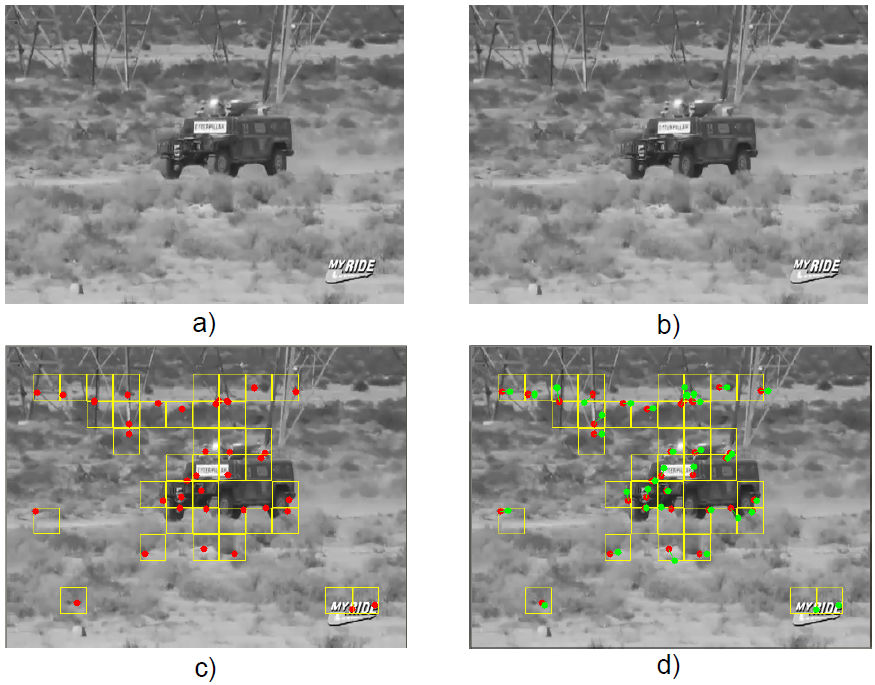
\includegraphics[scale=0.65]{img/3/of_example.png}
		\caption{Przykładowe wyznaczanie wektora przesunięcia -- źródło \cite{kryjak_14_vibe}}
		\label{fig:vibe_of_example}
	\end{figure}

\subsection{Detekcja narożników - metoda Harrisa-Stephensa}
\label{subsec:vibe_harris}

Algorytm detekcji narożników został opisany w publikacji \cite{harris_88}. 
Z punktu widzenia obliczeń opiera się on głównie na operacjach konwolucji. 
W pierwszej kolejności należy określić tzw. macierz Harrisa. 
Jej definicję przedstawia równanie (\ref{equ:vibe_harris_matrix}).

    \begin{equation}
        H = \begin{bmatrix}
               I_x^2 \otimes G    & I_x I_y \otimes G  \\
               I_x I_y \otimes G  & I_y^2 \otimes G    \\
     \end{bmatrix}
        \label{equ:vibe_harris_matrix}
    \end{equation}
gdzie:
\begin{eqwhere}[2cm]
	\item[$I_x,\, I_y$] pierwsza pochodna obrazu wejściowego (pozioma i pionowa)
	\item[$\otimes G$] operacja konwolucji -- wygładzenie obraz z wykorzystaniem filtru Gaussa
\end{eqwhere}

Pochodne pierwszego rzędu obrazu wejściowego są obliczane z wykorzystaniem filtru Prewitta, maska pozioma $P_x$ i pionowa $P_y$ zostały przedstawione równaniem (\ref{equ:vibe_prewitt}). 
Z kolei przykładowa maska filtru Gaussa (dla $\sigma = 3$) została opisana równaniem (\ref{equ:vibe_gauss}).

    \begin{equation}
        P_x = \begin{bmatrix}
			    -1 & 0 & +1 \\
			    -1 & 0 & +1 \\
			    -1 & 0 & +1 \\
		    \end{bmatrix}
		,\quad 
		P_y= \begin{bmatrix}
			    +1 & +1 & +1 \\
			    0 & 0 & 0 \\
			    -1 & -1 & -1 \\
		    \end{bmatrix}
        \label{equ:vibe_prewitt}
    \end{equation}

    \begin{equation}
       G(\sigma=3) = \begin{bmatrix}
			   0.1070 & 0.1131 & 0.1070 \\
			   0.1131 & 0.1196 & 0.1131 \\
			   0.1070 & 0.1131 & 0.1070 \\
		    \end{bmatrix}
        \label{equ:vibe_gauss}
    \end{equation}


Ostateczna odpowiedź detektora krawędzi wymaga obliczenia wyznacznika i śladu macierzy $H$. 
Finalna wartość może zostać zapisana równaniem (\ref{equ:vibe_harris_response}).
    \begin{equation}
        H_R = det(H)-k \cdot trace^2(H)
        \label{equ:vibe_harris_response}
    \end{equation}
gdzie: $k$ -- współczynnik skalowania (przyjmuje wartości \num{0.02} -- \num{0.2})


Po uwzględnieniu wzorów na wskaźnik i ślad macierzy o rozmiarze $2x2$, wzór (\ref{equ:vibe_harris_response}) można przekształcić do postaci (\ref{equ:vibe_harris_response_final}). 
Otrzymana wartość $H_R$ jest porównywana z~progiem. 
Jeżeli wartość $H_{TH}$ zostanie przekroczona dany piksel uznawany jest za narożnik obiektu.  

    \begin{equation}
        H_R = I_x^2 \otimes G \cdot I_y^2 \otimes G - (I_x I_y \otimes G)^2  - k \cdot (I_x^2 \otimes G + I_y^2 \otimes G)^2
        \label{equ:vibe_harris_response_final}
    \end{equation}

\subsection{Uwagi}
\label{subsec:vibe_uwagi}

Algorytm \textit{ViBE} jest metodą zawierającą niezbyt złożony model tła oraz charakteryzującą się niedużą złożonością obliczeniową. 
Warto jeszcze raz podkreślić niewielką liczbę parametrów -- ostateczna lista prezentują się następująco (w nawiasach podano wartości domyślne):\\
\-\hspace{1cm} $N$ -- liczba próbek w modelu tła ($20$)\\
\-\hspace{1cm} $\#_{min}$ -- minimalna liczba próbek wymagana w teście dopasowania ($2$)\\
\-\hspace{1cm} $R$ -- próg dopasowania próbki do modelu ($15$) \\
\-\hspace{1cm} $T$ -- prawdopodobieństwo wykonania aktualizacji ($\frac{1}{16}$)\\
\\
\noindent W przypadku rozszerzonej wersji algorytmu, należy uwzględnić jeszcze jeden dodatkowy parametr, mianowicie próg $H_{TH}$ (domyślnie $10$), wykorzystywany podczas detekcji narożników metodą Harrisa-Stephensa.
    

\section{Pixel-Based Adaptive Segmenter}
\label{sec:pbas_teoria}
%%TODO proszę podać referencję do oryginalnej wersji artykułu - jest w drugim akapicie

Omawiany algorytm jest rozszerzeniem opisanej rozdziale \ref{subsec:vibe_opis} metody \textit{ViBE}. 
\textit{PBAS} (ang. \textit{Pixel Based Adaptive Segmenter}, podobnie jak opisana już wcześniej metoda, także posiada model, który składa się między innymi z próbek pikseli pochodzących z poprzednich ramek obrazu. 
Dodatkowo, próg dopasowania oraz prawdopodobieństwo dokonania aktualizacji są niezależne i na bieżąco uaktualniane dla każdego modelu. 
Opisywany algorytm może zostać zaimplementowany zarówno w wersji \textit{RGB} jak i w skali szarości.

Algorytm został zaprezentowany w artykule \cite{kryjak_14_pbas} i to właśnie na jego podstawie powstał niniejszy opis. 
Oprócz standardowej wersji metody \textit{PBAS} autorzy zaproponowali także dodatkowy mechanizm eliminacji tzw. ,,duchów'' (opis tego zjawiska został dokładnie opisany w rozdziale \ref{subsec:pbas_duchy}). 
Zaproponowane rozwiązanie opiera się na algorytmie etykietowania obiektów i następnie porównywania krawędzi na obrazie wejściowym oraz masce wyjściowej w obrębie każdego z nich.


\subsection{Opis algorytmu}
\label{subsec:pbas_opis}

Model tła jest nieco bardziej złożony niż ten przedstawiony w algorytmie \textit{ViBE}. 
Jego pierwsza część, podobnie jak w poprzedniej metodzie, składa się z $N$ zapamiętanych próbek. 
W celu uproszczenia dalszego zapisu matematycznego, zdefiniujmy ten zbiór jako $B(x_i)$, gdzie $x_i$ to aktualnie przetwarzany piksel obrazu, całość została opisana równaniem (\ref{equ:pbas_model_1}).

	\begin{equation}
		B(x_i)= \left\{ B_1(x_i), B_2(x_i), \dotsc, B_N(x_i) \right\}
	\label{equ:pbas_model_1}	
	\end{equation}

Test dopasowania, jest również bardzo podobny do tego, który występuje w metodzie \textit{ViBE}. 
Jedyną różnicą jest niezależny dla każdego modelu próg przynależności do modelu $R(x_i)$, całość została przedstawiona równaniem (\ref{equ:pbas_test}).

	\begin{equation}
	    F(x_i) = 
		\begin{dcases}
    		1, & \text{gdy } \sum_{k=0}^{N} \{ d(I(x_i), B_k(x_i)) < R(x_i) \} < \#_{min} \\
    		0, & \text{w pozostałych przypadkach} 
		\end{dcases}
	\label{equ:pbas_test}	
	\end{equation}
\noindent gdzie $d$ to funkcja odległości pomiędzy próbką z modelu tła, a aktualnym pikselem. 

W przypadku algorytmu w wersji \textit{RGB} każdy kanał przetwarzany jest osobno z wykorzystaniem niezależnego modelu tła. 
Finalna maska jest alternatywą logiczną wyników z poszczególnych kanałów. 
Oznaczając poszczególne maski jako $F_R$, $F_G$, $F_B$ ostateczną klasyfikację możemy zapisać równaniem~(\ref{equ:pbas_final_mask}).

    \begin{equation}
        F_{RGB} = F_R \lor \lor F_G \lor F_B
    \label{equ:pbas_final_mask}
    \end{equation}


Ponieważ każdy kanał analizowany jest osobno, funkcję odległości pomiędzy próbkami można zapisać bardzo prosto równaniem (\ref{equ:pbas_dist}). Jest to po prostu moduł różnicy.
	\begin{equation}
		d(I(x_i),B_k(x_i)) = | I(x_i) - B_k(x_i) |
	\label{equ:pbas_dist}	
	\end{equation}

Kolejnym krokiem po przeprowadzeniu testu dopasowania i klasyfikacji piksela jest aktualizacja modelu tła. 
Zastosowano konserwatywne podejście, czyli aktualizowane są tylko piksele sklasyfikowane jako tło. 
Analogicznie jak w algorytmie \textit{ViBE} decyzja o aktualizacji podejmowana jest losowo. 
Prawdopodobieństwo jej wykonania wynosi $p = 1/T(x_i)$, gdzie parametr $T(x_i)$ jest dynamicznie aktualizowany i niezależny dla każdego piksela. Sama aktualizacja, polega na nadpisaniu, losowo wybranej próbki $B_k(x_i)$ z modelu aktualną wartością piksela $I(x_i)$. Dodatkowo, wybierany jest losowy piksela z otoczenia $3x3$ i losowo wybrana próbka z modelu mu odpowiadającego, jest nadpisywana wartością tego piksela. Wprowadzenie czynnika losowego, pozwala w pewnym stopniu wyeliminować negatywne skutki konserwatywnego podejścia do aktualizacji modelu.
%%TODO też napiać po co to

Niezależnie od aktualizacji części modelu zawierającej zapamiętane próbki dokonywana jest zmiana parametrów $R(x_i)$ i $T(x_i)$. 
W tym celu konieczne jest zdefiniowanie kolejnego elementu modelu tła, który zawiera zbiór minimalnych odległości pomiędzy próbką z modelu a aktualną wartością piksela. 
Zbiór ten został opisany równaniem (\ref{equ:pbas_model_2}). 
 
	\begin{equation}
		D(x_i)= \left\{ D_1(x_i), D_2(x_i) \dotsc, D_N(x_i) \right\}
	\label{equ:pbas_model_2}	
	\end{equation}

Przedstawiony zbiór $D(x_i)$ aktualizowany jest razem ze zbiorem próbek. 
Nadpisywany jest jedynie element o indeksie $k$ dla którego dystans pomiędzy próbką i aktualnym pikselem jest najmniejsza. 
Zostało to przedstawione równaniem (\ref{equ:pbas_d_min}).
	
	\begin{equation}
		d_{min}(x_i) = min_k d(I(x_i), B_k(x_i))
	\label{equ:pbas_d_min}	
	\end{equation}

Do aktualizacji progu dopasowania, czyli parametru $R(x_i)$ konieczne jest wyznaczenie tzw. miary dynamiki tła, czyli inaczej wartości średniej ze zbioru $D(x_i)$. 
Finalny wzór na nową wartość progu przedstawia równanie (\ref{equ:pbas_r_update}). 
Warto dodać, że przyjęto także dolne ograniczenie wartości parametru, wynoszące $R_{low} = 18$.
    
    \begin{equation}
	    R(x_i) = 
		\begin{dcases}
    		R(x_i)(1-R_{inc/dec}), & \text{jeżeli } R(x_i) > \bar{d}_{min}(x_i)R_{sc} \\
    		R(x_i)(1+R_{inc/dec}) & \text{w przeciwnym razie} 
		\end{dcases}
	\label{equ:pbas_r_update}	
	\end{equation}
gdzie:
\begin{eqwhere}[2.2cm]
	\item[$R_{inc/dec}$] stały współczynnik aktualizacji (domyślnie $0.05$)
	\item[$\bar{d}_{min}(x_i)$] wartość średnia zbioru $D(x_i)$
	\item[$R_{sc}$] współczynnik skalowania (domyślnie $5$)
\end{eqwhere}

Ostatni etap to aktualizacja parametru opisującego prawdopodobieństwo dokonania aktualizacji, czyli $T(x_i)$. 
Nowa wartość zależy od wyniku klasyfikacji piksela i została opisana równaniem (\ref{equ:pbas_t_update}). 
Przyjęto założenie, że parametr ten posiada także ograniczenie dolne jak i górne wynoszące odpowiednio $T_{low}=2$ i $T_{up}=200$.  

    \begin{equation}
	    T(x_i) = 
		\begin{dcases}
    		T(x_i) + \frac{T_{inc}}{\bar{d}_{min}(x_i)}, & \text{jeżeli } F(x_i)=1 \\
    		T(x_i) - \frac{T_{dec}}{\bar{d}_{min}(x_i)} & \text{w przeciwnym razie} 
		\end{dcases}
	\label{equ:pbas_t_update}	
	\end{equation}

%TODO mógłby być komentarz dlaczego takie podejście (ze zmiennymi R i T ) jest lepsze od stałych
Wartość $\bar{d}_{min}(x_i)$ określa dynamikę tła. W przypadku statycznego tła wartość ta będzie równa 0, natomiast jeżeli tło zawiera więcej dynamicznych elementów to będzie odpowiednio wyższa. Parametr ten jest wykorzystywany podczas dynamicznej aktualizacji parametru $R$, opisanej wzorem (\ref{equ:pbas_r_update}). Jak łatwo zauważyć, wzrost dynamiki tła, powoduje również delikatny wzrost progu $R$. W przypadku dynamicznego tła często dokonywana jest błędna klasyfikacja piksela jako pierwszoplanowego, z tego powodu zastosowano dynamiczną aktualizację parametru $T$ opisaną równaniem (\ref{equ:pbas_t_update}). Wartość jest podwyższa właśnie w sytuacji występowania dynamicznego tła w celu lepszego dostosowania modelu.

\subsection{Detekcja obiektów statycznych}
\label{subsec:pbas_duchy}

Autorzy publikacji \cite{kryjak_14_pbas} zaproponowali dodatkowy mechanizm eliminacji tzw. ,,duchów''. Przedstawiona metoda opiera się na porównaniu krawędzi na obrazie wejściowym i masce końcowej. 
%TODO tam nic nie było o modelu tła ??? - analizowane są krawedzie na wejsciu i wyjsciu + cfd 
Jeżeli układ krawędzi, na obu obrazach jest identyczny, to znaczy, że obiekt statyczny rzeczywiście istnieje, natomiast w przeciwnym wypadku jest on duchem i zostaje usunięty z finalnej maski. 
%%TODO trzeba jeszcze napisać, że to dotyczy obiektów statycznych...


Pierwszym krokiem, który należy wykonać w celu identyfikacji potencjalnych ,,duchów'' jest operacja odejmowania dwóch kolejnych ramek. 
W przestrzeni \textit{RGB} taka operacja jest opisana przez równanie (\ref{equ:pbas_cfd}).

    \begin{equation}
        dF(x_i) = \sum_{C \in \{R,G,B\}} | I(x_i)_{K}^C - I(x_i)_{K-1}^C |
    \label{equ:pbas_cfd}
    \end{equation}
    
\noindent gdzie przez $I(x_i)_{K}^C$ rozumiemy wartość jednej ze składowych \textit{R,G,B} piksela o położeniu $x_i$ w $K$-tej ramce obrazu.

Kolejny etap to obliczenie tzw. współczynnika stabilności. 
Operację tą opisuje równanie (\ref{equ:pbas_stability}). 
Jest ona wykonywana niezależnie dla każdego zidentyfikowanego obiektu na masce wyjściowej. 
Do tego celu konieczna jest także operacja indeksacji obiektów, ponieważ jest to zagadnienie dość złożone zostało ono opisane oddzielne w rozdziale \ref{subsec:pbas_indeksacja}. 
Sam współczynnik definiuje się jako stosunek liczby pikseli, których różnica opisana równaniem (\ref{equ:pbas_cfd}) przekracza ustalony próg $\theta$ do całkowitej powierzchni obiektu.

    \begin{equation}
        S_{O_k} = \frac{ \sum_{x_i \in O_k} dF(x_i) > \theta }{ \sum_{x_i \in O_k} F(x_i) }
    \label{equ:pbas_stability}
    \end{equation}
gdzie:
\begin{eqwhere}[2cm]
	\item[$O_k$] $k$-ty obiekt na masce wyjściowej, wyznaczony algorytmem indeksacji
	\item[$F(x_i)$] maska wyjściowa ze standardowego algorytmu \textit{PBAS}
\end{eqwhere}

\noindent Obiekt jest uznawany za statyczny (czyli potencjalnego ducha), jeżeli wartość współczynnika $S_{O_k}$ przekracza ustalony próg $S_{TH}$ (domyślnie równy $0.1$). 
Takie działanie ma na celu eliminację błędnej klasyfikacji wynikającej z szumów i zakłóceń obrazu.
%TODO no i dlatego,  ze duch z definicji jest statyczy


W celu weryfikacji, czy dany obiekt istniej zarówno na obrazie wejściowym jak i masce wyjściowej, użyty został mechanizm porównywania krawędzi.
Sama detekcja krawędzi została zrealizowana z wykorzystaniem filtru Sobela. 
Przykładowe maski dla osi $X$ i $Y$ przedstawiono w równaniu (\ref{equ:pbas_sobel}). 
Operacja konwolucji z maską Sobela realizowana jest osobno dla każdego kanału \textit{RGB}, następie obrazy wynikowe dla obu osi są sumowane i binaryzowanne ze stałym progiem $T_S$. 
Maska finalna stanowi alternatywę logiczną wyników z wszystkich kanałów.

    \begin{equation}
        S_x = \begin{bmatrix}
			    -1 & 0 & +1 \\
			    -2 & 0 & +2 \\
			    -1 & 0 & +1 \\
		    \end{bmatrix}
		,\quad 
		S_y = \begin{bmatrix}
			    +1 & +2 & +1 \\
			    0 & 0 & 0 \\
			    -1 & -2 & -1 \\
		    \end{bmatrix} 
    \label{equ:pbas_sobel}
    \end{equation}

Po wyznaczeniu krawędzi obrazu należy dla każdego obiektu obliczyć tzw. współczynnik podobieństwa krawędzi $EC_{O_k}$, został on przedstawiony za pomocą równania (\ref{equ:pbas_edge_coef}).  
Jeżeli otrzymana wartość przekracza próg $0.5$ oznacza to, że obiekt istnieje, czyli występuje zarówno na obrazie wejściowym jak i masce wyjściowej. 

    \begin{equation}
        EC_{O_k} = \frac{ \sum_{x_i \in O_k} F_E(x_i) == 1 \land I_E(x_i) == 1 }{ \sum_{x_i \in O_k} F_E(x_i) == 1 }
    \label{equ:pbas_edge_coef}
    \end{equation}
gdzie:
\begin{eqwhere}[2.2cm]
	\item[$F_E$] krawędzie na masce wyjściowej
	\item[$I_E$] maska zawierająca krawędzie na obrazie wejściowym
	\item[$O_k$] $k$-ty obiekt zidentyfikowany na masce wyjściowej
\end{eqwhere}

%TODO tu by się przydał rysunek tego interesu.... może być z któregoś artykułu

Schemat blokowy rozszerzonej wersji metody \textit{PBAS} został przedstawiony na rysunku \ref{fig:pbas_diagram}. 
Oprócz modułu obliczającego maskę pierwszoplanową z użyciem standardowego algorytmu \textit{PBAS} zawiera on dodatkowe bloki odpowiedzialne za wszystkie operacje opisane w niniejszym rozdziale. 
Moduł \textit{EDGE} służy do wyznaczania krawędzi na aktualnym obrazie wejściowym (oznaczonym jako $I_N$). 
Blok \textit{CFD} (ang. \textit{consecutive frame differencing}) oblicza różnicę dwóch ramek kolejnych ramek ($I_N$ i $I_{N-1}$) opisaną równaniem (\ref{equ:pbas_cfd}). 
Najbardziej złożonym elementem jest moduł \textit{CCA} (ang. \textit{Connected Component Analysis}). 
Jest w nim wykonywana indeksacja obiektów (opisana szczegółowo w rozdziale \ref{subsec:pbas_indeksacja}). 
Wartością końcową tej operacji są parametry prostokąta otaczającego zidentyfikowany obiekt (ang. \textit{bounding box}). 
Oprócz tego są wyznaczane wartości $S_{O_k}$ i $EC_{O_k}$ -- równania (\ref{equ:pbas_stability}) i (\ref{equ:pbas_edge_coef}) oraz finalna maska wyjściowa. 
Obliczone współczynniki stabilności i podobieństwa krawędzi są przekazywane jako sprzężenie zwrotne do standardowego algorytmu \textit{PBAS}.

 
	\begin{figure}[h]
		\centering
		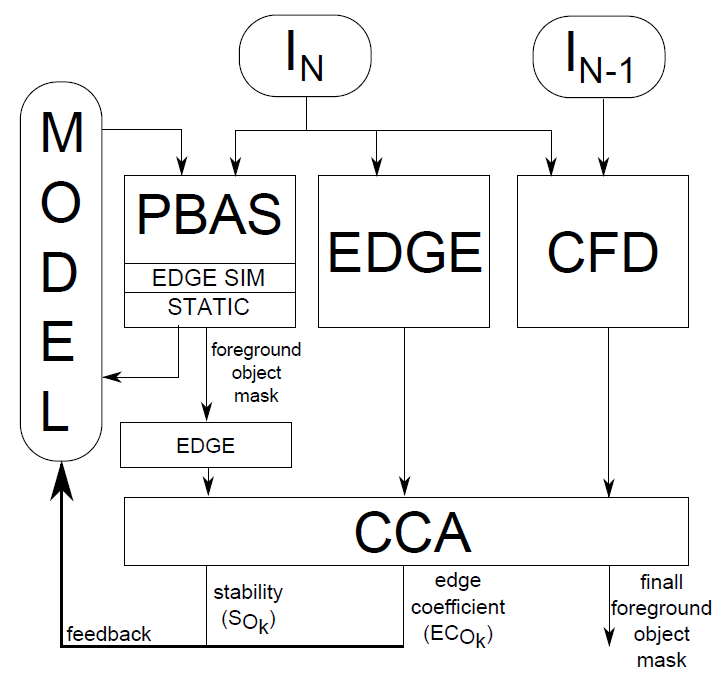
\includegraphics[scale=0.6]{img/3/pbas_diagram.png}
		\caption{Schemat blokowy rozszerzonej metody \textit{PBAS} -- źródło \cite{kryjak_14_pbas}}
		\label{fig:pbas_diagram}
	\end{figure}


Ostatnim krokiem jest obsługa sprzężenia zwrotnego, w tym celu do modelu tła zostały dodane dwa kolejne elementy. 
Pierwszym z nich jest licznik $S(x_i)_{cnt}$ określający przez ile ramek dany piksel był rozpoznawany jako obiekt statyczny. 
Sposób jego aktualizacji został opisany równaniem (\ref{equ:pbas_s_cnt}). 
    \begin{equation}
	    S(x_i)_{cnt} = 
		\begin{dcases}
    		S(x_i)_{cnt} + 1 & \text{jeżeli } S_{O_k} \geq  S_{TH}	 \\
            0                & \text{jeżeli } S_{O_k} <  S_{TH}	     \\		
    		S(x_i)_{cnt} - 1 & \text{w pozostałych przypadkach} 
		\end{dcases}
	\label{equ:pbas_s_cnt}	
	\end{equation}

\noindent Operacja ta jest przeprowadzana dla każdego piksela wewnątrz prostokąta otaczającego dany obiekt. Licznik jest inkrementowany dla obiektów zaklasyfikowanych jako statyczne, dla poruszających się zostaje wyzerowany, natomiast dla elementów tła jest dekrementowany.

Drugim dodatkowym elementem modelu jest średnia krocząca współczynnika podobieństwa krawędzi $EC(x_i)_{mean}$, jej wartość jest aktualizowana zgodnie z równaniem (\ref{equ:pbas_ec_mean}).

    \begin{equation}
	    EC(x_i)_{mean} = 
		\begin{dcases}
    		0.5EC(x_i) + 0.5EC(x_i)_{mean} & \text{jeżeli } S_{O_k} \geq  S_{TH} \land S(x_i)_{cnt} > S_{{cnt}_{TH}}	 \\
            1                & \text{w przeciwnym razie}		
		\end{dcases}
	\label{equ:pbas_ec_mean}	
	\end{equation}
\noindent gdzie poprzez $S_{{cnt}_{TH}}$ oznaczamy minimalną liczbę ramek przez którą obiekt musi pozostać statyczny.
\\
\noindent Opisane parametry są wykorzystywane w procesie aktualizacji modelu, niezależnie od decyzji podjętej według standardowej procedury, model zostaje zaktualizowany jeżeli spełniony jest warunek logiczny opisany równaniem (\ref{equ:pbas_plus_update}). W praktyce oznacza to, że aktualizowane zostają piksele 
    \begin{equation}
	    S_{O_k} \geq S_{TH} \land S(x_i)_{cnt} > S_{cnt_{TH}} \land EC(x_i)_{mean} < 0.5
	\label{equ:pbas_plus_update}	
	\end{equation}
	
	%TODO skomentować co to w praktyce oznacza ...


\subsection{Indeksacja obiektów}
\label{subsec:pbas_indeksacja}

Opisany w rozdziale \ref{subsec:pbas_duchy} mechanizm detekcji tzw. ,,duchów'' wymaga rozróżnienia poszczególnych obiektów na wynikowej masce binarnej. 
W celu osiągnięcia takiego rezultatu, konieczne jest zastosowanie algorytmu indeksacji. 
Istnieje kilka podejść do realizacji tego zadania. 
W niniejszej pracy zdecydowano się zastosować metodę jednoprzebiegową, ze względu na jej stosunkowo prostą implementację w układach \textit{FPGA}. Sam algorytm został dokładnie przedstawiony w publikacji \cite{kryjak_14_pbas}, natomiast problem realizacji na platformie sprzętowej został szerzej rozwinięty w rozdziale \ref{sec:fpga_pbas_plus}. %%TODO powt. imple... 

Działanie algorytmu polega na nadawaniu poszczególnym pikselom etykiet reprezentujących kolejne obiekty. 
Piksele z taką samą etykietą reprezentują ten sam obiekt. 
Oczekiwanym efektem końcowym, wymaganym w omawianym algorytmie jest pole oraz parametry prostokąta otaczającego każdy obiekt w danej ramce obrazu.
Prostokąt otaczający jest reprezentowany przez cztery liczby $[x_1,y_1,x_2,y_2]$, gdzie współrzędne z indeksem 1 oznaczają lewy górny róg prostokąta, natomiast te z indeksem 2 prawy dolny róg. 

Pierwszym krokiem w procesie indeksacji jest wygenerowanie sąsiedztwa na podstawie którego aktualnie analizowany piksel będzie klasyfikowany. 
Jako sąsiedztwo, rozumie się najbliższe otaczające piksele. 
Ze względu na potokowe przetwarzanie obrazu wystarczy rozpatrzyć trzy piksele, znajdujące się w wyższym rzędzie oraz sąsiada po lewej stronie w rzędzie aktualnie analizowanym. 
Po wyznaczeniu sąsiedztwa, można przystąpić do klasyfikacji piksela. 
Jeżeli piksel ma wartość $1$ (jest elementem pierwszego planu) należy mu przypisać etykietę.  

Podczas operacji przypisania etykiety kolejnemu pikselowi mogą wystąpić trzy przypadki. 
Najprostszy z nich jest wtedy, gdy żaden z sąsiadujących pikseli nie ma przypisanej żadnej etykiety. 
W takiej sytuacji aktualny piksel traktowany jest jako fragment nowego obiektu i dostaje nową etykietę. 
Drugi przypadek to taki, w którym co najmniej jeden piksel posiada już przypisaną etykietą. 
Jeżeli pośród sąsiednich pikseli pojawia się tylko jedna etykieta oznacza to, że aktualny piksel także jest fragmentem obiektu oznaczonego właśnie tą etykietą, więc zostaje mu ona przypisana.
Ostatnim przypadkiem jest tzw. konflikt. 
Występuje on wtedy, gdy pośród sąsiednich pikseli występują różne etykiety. 
Taka sytuacja może się przytrafić na przykład w sytuacji gdy analizowany jest obiekt w kształcie litery V. 
Warto zauważyć, że w obszarze tego samego sąsiedztwa mogą istnieć tyko dwie różne etykiety. 
%%TODO to nie ma zwiazku z potokowością. Po prostu dla takiego sąsiedztwa nie może być inaczej...
W przypadku wystąpienia kolizji oba obiekty łączone są w jeden.
%%TODO to proszę jakieś odniesienie do literatury, skoro tego Pan jakoś bardziej nie opisuje.

Oprócz nadawania etykiet dla poszczególnych pikseli, na bieżąco aktualizowane jest także pole oraz parametry prostokąta otaczającego każdy do tej pory zidentyfikowany obiekt. %%TODO co to jest blok otaczający ??? chyba prostokąt tak samo obszar, cvhyba pole. POza tym jakoś trzeba wprowadzić, że oprócz nadawania etykliet.... 
W przypadku nowego obiektu, pole inicjializowane jest oczywiście wartością 1~natomiast współrzędne wierzchołków prostokąta otaczającego przyjmują współrzędne piksela. %%TODO blok
Dalsza aktualizacja pola obiektu wymaga jedynie inkrementacji wartości wraz z kolejnymi pikselami przypisanymi do danego obiektu. Prostokąt otaczający jest natomiast aktualizowany na podstawie współrzędnych $x$ i $y$ aktualnego piksela, zgodnie z równaniem~(\ref{equ:labeling_bbox_update}). %%TODO blok

    \begin{equation}
        (x_{1}, y_{1}, x_{2}, y_{2})= (min(x_{1}, x), min(y_{1}, y), max(x_{1}, x), max(y_{1}), y)
    \label{equ:labeling_bbox_update}
    \end{equation}

\noindent
W przypadku wystąpienia konfliktu, pola obu obiektów zostają zsumowane. Parametry nowego prostokąta otaczającego dobierane są tak, aby pokrył on oba wcześniejsze prostokąty. Spośród współrzędnych lewych górnych rogów obu łączonych obiektów, wybierane są wartości mniejsze i zostają ustawione jako współrzędne lewego rogu nowego prostokąta. W przypadku prawego dolnego rogu postępowanie jest analogiczne, tylko wybierane są wartości większe.
%%TODO ale czego ???

%Do zaprezentowania pełnego zapisu matematycznego przyjęto następujące oznaczenia, niech $I$ oznacza obraz binarny z którego chcemy wyodrębnić poszczególne obiekty, zbiór $F$ zawiera wszystkie piksele białe (pierwszoplanowe), natomiast zbiór $B$ czarne (reprezentujące tło). Obiektem nazywamy z kolei zbiór $C$, będący podzbiorem $F$, taki że wszystkie piksele są połączone. Dwa piksele $P$ i $Q$ są połączone, jeżeli istnieje ścieżka utworzona z pikseli $(p_0, p_1, \dotsc , p_n)$, taka że $p_0=P$, $p_n=Q$ i każdy kolejny piksel jest sąsiadem poprzedniego. W tym przypadku przez sąsiedztwo rozumiane jest $8$ pikseli otaczających.%

\subsection{Uwagi}
\label{subsec:pbas_uwagi}

Przedstawiony algorytm jest rozszerzoną wersją omówionej w rozdziale \ref{sec:vibe_teoria} metody \textit{ViBE}. 
W tym przypadku wykorzystywany jest bardziej rozbudowany model tła, a sam algorytm charakteryzuje się większą złożonością obliczeniową. 
W stosunku do wcześniej omawianej metody, zwiększyła się także lista parametrów, kompletna lista została zamieszczona poniżej (w nawiasach umieszczono wartości domyślne):\\
\-\hspace{1cm} $N$ -- liczba próbek w modelu tła ($19$)\\
\-\hspace{1cm} $\#_{min}$ -- minimalna liczba próbek wymagana w teście dopasowania ($2$)\\
\-\hspace{1cm} $R_{init}$ -- początkowa wartość progu dopasowania próbki do modelu ($30$) \\
\-\hspace{1cm} $T_{init}$ -- początkowe prawdopodobieństwo wykonania aktualizacji ($\frac{1}{16}$)\\
\-\hspace{1cm} $R_{low}$ -- dolne ograniczenie progu dopasowania próbki do modelu ($18$) \\
\-\hspace{1cm} $T_{low}, \, T_{up} $ -- dolne i górne ograniczenie progu dopasowania próbki do modelu ($2$ i $200$) \\
\-\hspace{1cm} $R_{inc/dec}$ -- współczynnik wykorzystywany przy aktualizacji parametru $R$ (\num{0.05}) \\
\-\hspace{1cm} $R_{SC}$ -- współczynnik skalowania wykorzystywany przy aktualizacji parametru $R$ ($5$)\\
\\
\noindent W rozszerzonej wersji, zawierającej mechanizm detekcji duchów, należy uwzględnić jeszcze następujące parametry:\\
\-\hspace{1cm} $\theta$ -- próg wykorzystywany w (\ref{equ:pbas_stability}), określający ruchome obiekty ($50$)\\
\-\hspace{1cm} $S_{TH}$ -- wartość progowa współczynnika stabilności (\num{0.01})\\
\-\hspace{1cm} $S_{cnt_{TH}}$ -- minimalna liczba ramek przez która obiekt musi pozostać statyczny ($5$) \\
\-\hspace{1cm} $T_{S}$ -- próg binaryzacji wykorzystywany w detekcji krawędzi metodą Sobela ($50$)\\

%TODO Tak sobie jeszcze myślę, że pod każdą metodą warto napisać z czego składa się model tła - przygotowanie pod analize sposóbu dostępu do pamięci. - mysle, że w przypadku ViBE oraz GMM jest to wystarczajco dobrze opisane na poczatku
Kompletny model tła dla pojedynczego piksela składa się z $N$ zapamiętanych próbek (\ref{equ:pbas_model_1}), $N$-elementowego zbioru minimalnych odległości pomiędzy próbką a pikselem (\ref{equ:pbas_model_2}) oraz parametrów $R$ i $T$. W przypadku rozszerzonej wersji algorytmu należy jeszcze uwzględnić dodatkowy licznik $S(x_i)_{cnt}$ (\ref{equ:pbas_s_cnt}), współczynnik podobieństwa krawędzi $EC(x_i)_{mean}$ (\ref{equ:pbas_ec_mean}) oraz poprzednią wartość piksela konieczną do obliczenia różnicy dwóch kolejnych ramek.


\section{Gaussian Mixture Models}
\label{sec:gmm_teoria}

Metoda \textit{GMM} (ang. \textit{Gaussian Mixture Models}) jest algorytmem wykorzystującym statystyczny model tła. 
%TODO podać, że jeszcze MOG (mixture of gaussian)
W przeciwieństwie do algorytmów opisywanych w poprzednich rozdziałach, tutaj model tła nie składa się z zapamiętanych próbek. 
Podobnie jak inne metody, ta także może przetwarzać obraz w różnych przestrzeniach barw. 

Jako, że jest to algorytm opublikowany po raz pierwszy w 1999 roku \cite{Stauffer_Grimson_99}, to od tamtej pory doczekał się wielu różnych odmian i udoskonaleń. %%TODO algorytm doczekała ????
Ponieważ tematem niniejszej pracy jest analiza i unifikacja algorytmów opracowanych w Laboratorium Biocybernetyki AGH w tym rozdziale zostanie zamieszczony opis powstały w oparciu o prace inżynierskie \cite{janus_15, piszczek_15}. W wyżej wymienionych publikacjach zamieszczono wyczerpujący opis metody, zarówno od strony teoretycznej jak i implementacyjnej. Niniejsza praca zawiera jedynie podstawowe założenia i główne kroki algorytmu.


\subsection{Opis Algorytmu}
\label{subsec:gmm_opis}


Opisywany algorytm opiera się na modelu tła składającym się z $K$ rozkładów Gaussa. 
Są one podzielone na dwie grupy -- część z nich reprezentuje tło, reszta obiekty pierwszoplanowe. 
Model skonstruowany jest tak, że dla każdego piksela zdefiniowany jest osobny zestaw rozkładów Gaussa, który następnie jest niezależnie aktualizowany. 
Niewątpliwą zaletą w kontekście implementacji w układzie \textit{FPGA} jest brak jakichkolwiek operacji wykorzystujących otoczenie piksela. 
Pozwala to zaoszczędzić dużą część zasobów. 
Szczegóły implementacji sprzętowej przedstawiono w rozdziale \ref{sec:fpga_gmm}.

Każdy rozkład Gaussa składa się z trzech elementów: wagi ($\omega$), wariancji ($\sigma$) i wartości średniej ($\mu$). 
W przypadku przetwarzania obrazu w przestrzeni \textit{RGB}, w celu uproszczenie obliczeń, zakłada się, że waga i wariancja jest identyczna dla wszystkich trzech kanałów. 
Opierając się na publikacjach \cite{Stauffer_Grimson_99, piszczek_15}, liczbę rozkładów (parametr $K$) najlepiej przyjąć z zakresu $3$ -- $5$.  


Pierwszym krokiem jest posortowanie rozkładów Gaussa według współczynnika $r_i = \frac{\omega_i}{\sigma_i}$ w kolejności rosnącej (przez $i$ rozumiemy numer rozkładu, natomiast $\omega_{i,t}$ oznacza wagę i-tego rozkładu w czasie t). 
Ze względu na przyjęte uproszczenie, że wariancja jest identyczna dla wszystkich kanałów RGB, macierz kowariancji i-tego rozkładu w chwili t może zostać zapisana równaniem (\ref{equ:gmm_cov}).

    \begin{equation}
        \Sigma_{i,t} = \sigma_{i,t}^2 I
    \label{equ:gmm_cov}
    \end{equation}

Zastosowanie sortowania według współczynnika $r_i$ powoduje umieszczenie na początku listy tych rozkładów, które najprawdopodobniej reprezentują tło (czyli tych o najwyższej wadze oraz najniższej wariancji). 
Przyjęto, że pierwsze $B$ rozkładów z listy uznaje się za rozkładu reprezentujące tło, kolejne to już obiekty pierwszoplanowe. 
Jak łatwo zauważyć, rozkłady przedstawiające tło, mają zdecydowanie wyższą wagę oraz niewielką wariancję. 
Równanie (\ref{equ:gmm_b}) określa wartość $B$, jest to liczba rozkładów, dla których suma wag przekracza próg $T$.


    \begin{equation}
        B = arg\,min_b \left(\sum_{i=1}^{b} \omega_{i,t} > T\right)
    \label{equ:gmm_b}
    \end{equation}

Kolejnym etap to test dopasowania nowego piksela do modelu. 
Przeprowadzany jest on dla każdego rozkładu Gaussa z posortowanej listy i~przerywany w momencie uzyskania pozytywnego wyniku (piksel wejściowy pasuje do modelu). 
Jeżeli przyjmiemy, że nowy piksel pojawia się w chwili $t+1$ to test dopasowania przeprowadzany jest z modelem z~chwili $t$. 
Pozytywny wynik testu określa zależność (\ref{equ:gmm_mahalanobis}).

    \begin{equation}
        \sqrt{ \left( \left( X_{t+1} - \mu_{i,t} \right)^T \cdot \Sigma_{i,t}^{-1} \cdot \left( X_{t+1} - \mu_{i,t} \right) \right)} < k \sigma_{i,t}
    \label{equ:gmm_mahalanobis}
    \end{equation}

\noindent gdzie próg $k$ domyślnie przyjmuje wartość \num{2.5}


Na tym etapie algorytmu, należy rozważyć dwa przypadki. 
Jeżeli piksel wejściowy został dopasowany do jednego z $K$ rozkładów Gaussa, to zostaje on klasyfikowany na podstawie wcześniejszej przynależności danego rozkładu, zgodnie z (\ref{equ:gmm_b}). 
Podczas aktualizacji modelu, zostanie wykorzystany parametr $\alpha$ określający stałą uczenia. 
Parametry rozkładu Gaussa, który przeszedł test dopasowania określony równaniem (\ref{equ:gmm_mahalanobis}), zostaje zaktualizowany według zależności (\ref{equ:gmm_w_update}), (\ref{equ:gmm_u_update}) i (\ref{equ:gmm_sigma_update}).

    \begin{equation}
        \omega_{i, t+1} = (1-\alpha)\omega_{i,t} + \alpha
    \label{equ:gmm_w_update}
    \end{equation}

    \begin{equation}
        \mu_{i, t+1} = (1-\rho)\mu_{i,t} + \rho X_{t+1}
    \label{equ:gmm_u_update}
    \end{equation}

    \begin{equation}
        \sigma_{i, t+1}^2 = (1-\rho)\sigma_{i,t}^2 + \rho (X_{t+1} - \mu{i,t+1})(X_{t+1} - \mu{i,t+1})^T
    \label{equ:gmm_sigma_update}
    \end{equation}

\noindent Do przedstawienia funkcji $\rho$ konieczna jest także definicja funkcji gęstości prawdopodobieństwa, która jest opisana równaniem (\ref{equ:gmm_density}). 
Z kolei samą funkcję $\rho$ przedstawia równanie (\ref{equ:gmm_rho}).

    \begin{equation}
        \eta (X_t, \mu, \Sigma) = \frac{1}{(2\pi)^{n/2} |\Sigma|^{1/2}} e^{-\frac{1}{2} (X_t - \mu)\Sigma^{-1} (X_t - \mu)} 
    \label{equ:gmm_density}
    \end{equation}
gdzie:
\begin{eqwhere}[2cm]
	\item[$X_t$] wartość piksela w chwili t
	\item[$\mu$] wektor wartości średnich rozkładu Gaussa
	\item[$\Sigma$] macierz kowariancji -- wzór (\ref{equ:gmm_cov})\\
\end{eqwhere}


    \begin{equation}
        \rho = \alpha \eta(X_{t+1}, \mu_{i}, \Sigma_{i})
    \label{equ:gmm_rho}
    \end{equation}

Reszta rozkładów, która nie przeszła testu dopasowania, zostaje zaktualizowana według równania (\ref{equ:gmm_unmatched_update}), nadpisywana jest tylko waga, wartość średnia i wariancja pozostają niezmienione.

    \begin{equation}
        \omega_{j,t+1} = (1-\alpha)\omega_{j,t}
    \label{equ:gmm_unmatched_update}
    \end{equation}

Drugim przypadek to piksel niepasujący do żadnego rozkładu. 
W takiej sytuacji jest on automatycznie klasyfikowany jako element pierwszoplanowy. 
Aktualizacja modelu w tym przypadku polega na zastąpieniu rozkładu o najniższej wadze nowym. 
Sama waga pozostaje niezmieniona, natomiast aktualna wartość piksela zapisywana jest jako wartość średnia. Przypisywana jest także duża wariancja inicjalizująca, która jest określona globalnie jako parametr całego algorytmu. \\

Warto jeszcze raz nadmienić, że powyższe operacje wykonywane są cyklicznie dla każdego piksela z wykorzystaniem niezależnego modelu tła. 
Lista wszystkich parametrów algorytmu \textit{GMM} przedstawia się następująco: \\
\-\hspace{1cm} $K$ -- liczba rozkładów Gaussa\\
\-\hspace{1cm} $T$ -- próg z przedziału $0$--$1$ pozwalający rozgraniczyć rozkłady tła i pierwszoplanowe\\
\-\hspace{1cm} $k$ -- współczynnik używany w teście dopasowania (\ref{equ:gmm_mahalanobis})\\
\-\hspace{1cm} $\alpha$ -- współczynnik uczenia z przedziału $0$--$1$\\
\-\hspace{1cm} $\sigma_{init}$ -- wariancja, którą inicjalizowany jest nowy gaussian\\ 


\subsection{Uwagi}
\label{subsec:gmm_uwagi}

Algorytm opisany w niniejszym rozdziale, przedstawia nieco odmienne podejście do segmentacji obiektów pierwszoplanowych w stosunku do metod opisanych wcześniej. 
Jak już zostało wspomniane w rozdziale \ref{cha:przeglad_metod} algorytm \textit{GMM} jest bardzo rozległym zagadnieniem, będącym przedmiotem badań wielu publikacji \cite{Stauffer_Grimson_99, Genovese_Napoli_13, piszczek_15, wang_14}. 
Ze względu na skomplikowane operacje matematyczne z punktu widzenia układów \textit{FPGA}, sama implementacja również jest dość złożonym problemem.

Jak słusznie zauważyli autorzy przytoczonych publikacji, algorytm \textit{GMM} zapewnia zadowalające rezultaty, aczkolwiek jest bardzo podatny na różnego rodzaju zakłócenia, szumy i zmiany oświetlenia. 
Mimo to w większość przypadków, jest to metoda, mogąca z powodzeniem zostać wykorzystana jako samodzielny system segmentacji tła.  

%%TODO A opis FTSG ??? choćby skrócony i na podstawie pracy inżynierskiej ? dla kompletności 
\section{Algorytm Flux Tensor with Split Gaussian Models}
\label{sec:ftsg}

Metoda \textit{FTSG}, jak zostało wspomniane w rozdziale \ref{sec:model_inne}, po raz pierwszy opisano w publikacji \cite{wang_14}, jej niepełną wersję zaimplementowano także w ukłądzie \textit{FPGA} w ramach pracy inżynierskiej \cite{janus_15}. Jest to algorytm hybrydowy, łączący metodę \textit{Flux Tensor} (opisaną w podrozdziale \ref{subsec:flux_tensor_opis}) oraz zmodyfikowaną metodą \textit{GMM}, nazwaną \textit{Split Gaussian Models} (podrozdział \ref{subsec:split_gaussian_opis}). Zamieszczony w niniejszym rozdziale opis powstał w oparciu o wspomnianą pracę dyplomową, również zrealizowaną w Laboratorium Biocybernetyki AGH.

Oba wykorzystane algorytmy zawierają pewne wady, jednak w teorii powinny doskonale się uzupełniać, co skłoniło autorów publikacji do ich jednoczesnego wykorzystania. Metoda \textit{Flux Tensor} umożliwia jedynie wykrywanie obiektów ruchomych, dodatkowo jednak zapewnia bardzo dobrą eliminację zakłóceń spowodowanych zmianami oświetlenia. Przeciwieństwem takiego podejścia jest druga wykorzystana metoda, która będąc bardziej podatną na zakłócenia, umożliwia również detekcję obiektów statycznych.

\subsection{Algorytm Flux Tensor}
\label{subsec:flux_tensor_opis}

Metoda \textit{Flux Tensor} jest uniwersalnym algorytmem, służącym do wykrywania ruchomych obiektów na obrazie ze statycznie umiejscowionej kamery. Oprócz zastosowania a algorytmie \textit{FTSG}, metoda ta oraz jej implementacja sprzętowa została opisana między innymi w publikacji \cite{janus_16_flux}. Idea tego podejścia opiera się na detekcji krawędzi na obrazie wejściowym oraz wyznaczaniu pochodnej tego obrazu po czasie. Następnie, na podstawie tych dwóch informacji dokonywana jest identyfikacja ruchomych obiektów.

W opisywanym wariancie, algorytm operuje jedynie na obrazie w skali szarości. Przyjmijmy następujące oznaczenia: $x$, $y$ -- współrzędne piksela na obrazie, $t$ -- czas, wektor w przestrzeni $(x,y,t)$ zapiszmy jako $v$, natomiast wartość piksela wejściowego jako $I(v)$. Kolejnym krokiem jest zdefiniowanie macierzy \textit{Flux Tensor}, opisującej zmiany wartości piksela wejściowego w lokalnej czasoprzestrzeni. Oznaczmy przez $\Omega$ otoczenie w przestrzeni $(x,y,t)$, które jest rozważane przy analizie danego piksela. Macierz \textit{Flux Tensor} została opisana równaniem (\ref{equ:flux_matrix}).

\begin{equation}
			J_F(i) = 
			\begin{pmatrix}
			\int_\Omega \left(\frac{\partial^2 I(v)}{\partial x\partial t}\right)^2\,dv & 
			\int_\Omega \frac{\partial^2 I(v)}{\partial x\partial t}\frac{\partial^2 I(v)}{\partial y 							\partial t}\,dv & 
			\int_\Omega \frac{\partial^2 I(v)}{\partial x\partial t}\frac{\partial^2 I(v)}{\partial^2 t}						\,dv	\\
			
			\int_\Omega \frac{\partial^2 I(v)}{\partial y\partial t}\frac{\partial^2 I(v)}{\partial x 							\partial t}\,dv & 
			\int_\Omega \left(\frac{\partial^2 I(v)}{\partial y\partial t}\right)^2\,dv & 
			\int_\Omega \frac{\partial^2 I(v)}{\partial y\partial t}\frac{\partial^2 I(v)}{\partial^2 t}						\,dv \\
			
			\int_\Omega \frac{\partial^2 I(v)}{\partial^2 t}\frac{\partial^2 I(v)}{\partial x\partial t}						\,dv & 
			\int_\Omega \frac{\partial^2 I(v)}{\partial^2 t}\frac{\partial^2 I(v)}{\partial y\partial t}						\,dv & 
			\int_\Omega \left(\frac{\partial^2 I(v)}{\partial^2 t}\right)^2\,dv \\		
			\end{pmatrix}
\label{equ:flux_matrix}
\end{equation}

Następnym etapem jest wyznaczenie śladu (sumy elementów na przekątnej) opisanej macierzy. Na tej podstawie dokonywana jest ostateczna klasyfikacja piksela. Jeżeli otrzymana wartości jest większa od wartości progowej $T$, to piksel zostaje uznany za ruchomy. W przeciwnym wypadku zakładamy, że jest to element statyczny. Przyjmijmy uproszczone oznaczenia:

\begin{equation}
	I_{xt}=\frac{\partial^2I(x,y,t)}{\partial x\partial t},\quad I_{yt}=\frac{\partial^2I(x,y,t)}{\partial y			\partial t},\quad I_{tt}=\frac{\partial^2I(x,y,t)}{\partial^2 t}	
\label{equ:flux_components}
\end{equation}

Wykorzystując zależności opisane w (\ref{equ:flux_components}), ślad macierzy można zapisać równaniem:

\begin{equation}
	trace(J_F) = \int_\Omega \left(I_{xt}^2(i) + I_{yt}^2(i) + I_{tt}^2(i)\right)\,dv
\label{equ:flux_trace}
\end{equation}

Wszystkie elementy koniecznie do wyliczenia wartości danej równaniem (\ref{equ:flux_trace}) są wyznaczane przy użyciu operacji konwolucji. Do obliczania składowej $I_{xt}$ wykorzystuje się filtry różniczkujące dla składowych $x$ i $t$, oraz filtr wygładzający dla składowej $y$. Analogicznie, w przypadku $I_{yt}$ używany jest filtr wygładzający dla składowej $x$. Ostatnim elementem jest składowa $I_{tt}$. Tutaj wykorzystuje się filtr wygładzający dla składowych $x$ i $y$. W operacji całkowania wykorzystuje się natomiast jednowymiarowe filtry uśredniające. Schemat ilustrujący wszystkie etapy został przedstawiony na rysunku \ref{fig:flux_operation_flow}.

    \begin{figure}[h!]
	\centering
	    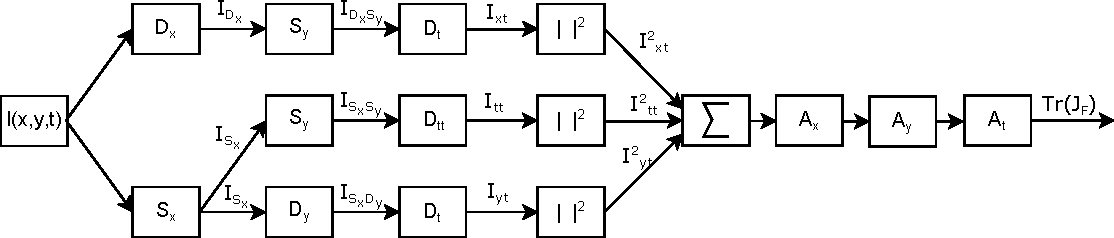
\includegraphics[scale=0.8]{img/3/flux_operation_flow.pdf}
	    \caption{Schemat operacji wyznaczających ślad macierzy $J_F$ -- źródło \cite{janus_15}}
	\label{fig:flux_operation_flow}
    \end{figure} 

\noindent Przedstawione na rysunku \ref{fig:flux_operation_flow} operacje oznaczają odpowiednio: 
\begin{eqwhere}[2cm]
	\item[$Dx$,\  $Dy$] filtry różniczkujące odpowiednio dla składowych $x$ i $y$
	\item[$Sx$,\  $Sy$] filtry wygładzające dla składowych $x$ i $y$
	\item[$Dt$,\  $Dtt$] odpowiednio pierwsza i druga pochodna z wartości piksela po czasie
	\item[$Ax$,\  $Ay$] filtry uśredniające przestrzenne
	\item[$At$] filtr uśredniający czasowy\\
\end{eqwhere}

Wygładzanie obrazu został zrealizowane poprzez filtr Gaussa ($\sigma = 3$). Różniczkę, w zależności od dobranej szerokości filtra, wyznacza się z wykorzystaniem następujących masek:
\begin{eqwhere}[2cm]
	\item[$n=3$] [$-\frac{1}{2}$, $0$, $\frac{1}{2}$]
	\item[$n=5$] [$\frac{1}{12}$, $-\frac{2}{3}$, $0$, $\frac{2}{3}$, $-\frac{1}{12}$]
	\item[$n=7$] [$-\frac{1}{60}$, $\frac{3}{20}$, $-\frac{3}{4}$, $0$, $\frac{3}{4}$, $-\frac{3}{20}$, $\frac{1}{60}$]\\
\end{eqwhere}

Po dokonaniu pewnych uproszczeń i założenia, że maski dla osi $x$ i $y$ mają identyczne rozmiary, można przedstawić finalną listę parametrów algorytmu:
\begin{eqwhere}[2cm]
	\item[$T$]	 wartość progowa
	\item[$nDs$]  rozmiar filtrów przestrzennych (różniczkujących i wygładzających)
	\item[$nDt$]  liczba ramek używana do różniczkowania po czasie
	\item[$nAs$]  rozmiar masek uśredniających przestrzennych
	\item[$nAt$]  liczba ramek używana do uśredniania po czasie\\
\end{eqwhere}

\subsection{Algorytm Split Gaussian Models}
\label{subsec:split_gaussian_opis}

Metoda \textit{Split Gaussian Models} opisana w \cite{janus_15} to zmodyfikowana wersja algorytmu \textit{GMM}. Zamiast jednego zestawu rozkładów Gaussa, składającego się z $K$ elementów, zdecydowano się wykorzystać dwa osobne modele, jeden reprezentujący tło i drugi pierwszoplanowy. Pierwszy z nich składa się ze zmiennej liczby rozkładów, natomiast drugi zawiera tylko jeden rozkład Gaussa. Test dopasowania do modelu tła uznawany jest za pozytywny, jeżeli piksel pasuje do chociaż jednego z rozkładów znajdujących się w modelu. W przypadku modelu pierwszoplanowego, piksel uznawany jest za element pierwszego planu jeżeli pasuje do rozkładu, w przeciwnym razie jest klasyfikowany jako element tła. Sam test dopasowania przeprowadzany jest identycznie jak w przypadku standardowej metody \textit{GMM}, przy użyciu wzoru (\ref{equ:gmm_mahalanobis}).

Oprócz definicji rozkładów Gaussa zmieniony został również proces aktualizacji modeli. Aktualizacja modelu tła wykonywana jest tylko wtedy, gdy piksel został sklasyfikowany jako tło. Analogicznie warunkiem aktualizacji modelu pierwszego planu jest sklasyfikowanie piksela jako pierwszoplanowego. Ostateczna decyzja o klasyfikacji piksela podejmowana jest po dokonaniu fuzji obu algorytmów, procedura ta została szczegółowo opisana w rozdziale \ref{subsec:ftgs_fuzja}. Dodatkowo wprowadzono także próg $T_l$, rozkłady których waga osiągnie wartość niższą od tego progu zostają usunięte.

Dwa równolegle działające modele dają także możliwość wykorzystania dwóch zestawów parametrów. W tym przypadku najistotniejsza jest stała uczenia $\alpha$. W celu lepszej detekcji obiektów statycznych, jej wartość dla modelu tła powinna być jak najmniejsza. Odwrotna sytuacja występuje w przypadku modelu pierwszego planu, tutaj wskazana jest wyższa wartość, gdyż pozwala to częściowo zniwelować efekt duchów. Dodatkowo można także manipulować stałą $k$ wykorzystywaną w teście dopasowania (\ref{equ:gmm_mahalanobis}). Dla modelu tła przyjmuje się zazwyczaj $k=3$, natomiast w modelu pierwszoplanowym, optymalna wartość to $k=20$. 

\section{Fuzja metody Flux Tensor i Split Gaussian Models}
\label{sec:ftsg_fuzja}

Schemat przedstawiający sposób połączenia obu algorytmów został zaprezentowany na rysunku \ref{fig:ftsg_flow}. Do analizy obrazu wykorzystywane są jednocześnie trzy modele: \textit{Flux Tensor}, model tła ze zmienną liczbą rozkładów Gaussa oraz model pierwszoplanowy zawierający jeden rozkład Gaussa. W pierwszym etapie analizowany jest wynik jedynie z dwóch pierwszych modułów. Finalna maska binarna została zapisana równaniem (\ref{equ:ftsg_final_mask}).

\begin{equation}
    F= 
\begin{dcases}
    1,   & \text{gdy }  F_F = 1 \land F_B = 1\\
    0,   & \text{gdy }  F_B = 0\\ 
    F_S, & \text{gdy }  F_F = 0 \land F_B = 1\\
\end{dcases}
\label{equ:ftsg_final_mask}
\end{equation}
gdzie:
\begin{eqwhere}[2cm]
	\item [$F_F$] maska otrzymana z modelu \textit{Flux Tensor}
	\item [$F_B$] maska otrzymana z modelu tła
	\item [$F_S$] maska definiująca obszar statyczny \\
\end{eqwhere}

		\begin{figure}[h]
				\centering
				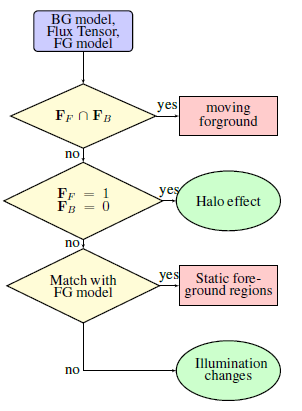
\includegraphics[scale=0.8]{img/3/ftsg_flow.png}
				\caption{Schemat operacji algorytmu \textit{FTSG} -- źródło \cite{wang_14}}
				\label{fig:ftsg_flow}
		\end{figure}

W sytuacji, gdy wynik klasyfikacji dla obu metod jest identyczny, sprawa ostatecznej przynależności jest oczywista. Piksel zostaje uznany za obiekt jeżeli $F_F = 1 \land F_B = 1$ lub za statyczne tło ($F_F = 0 \land F_B = 0$). Jeżeli wyniki obu modeli są sprzeczne konieczna jest dodatkowa analiza. Prostszy przypadek występuje w sytuacji, gdy metoda \textit{Flux Tensor} oznaczy piksel jako element pierwszego planu i jednocześnie pasuje on do modelu tła. Ostatecznie piksel klasyfikowany jest wtedy jako tło. Taka decyzja jest podejmowana, ponieważ algorytm \textit{Flux Tensor} zawsze zaznacza obiekty o trochę większym obszarze niż są one w rzeczywistości (tzw.~efekt halo). Z uwagi na fakt, że metoda wykorzystująca rozkłady Gaussa wykrywa zarówno obiekty statyczne jak i ruchome, nie występuje ryzyko utraty danych.

Bardziej skomplikowana jest sytuacja odwrotna, czyli $F_F = 0 \land F_B = 1$. Tutaj konieczne jest wykorzystanie modelu pierwszoplanowego i na jego podstawie podejmowana jest ostateczna decyzja. Jeżeli piksel pasuje do modelu to zostaje zaklasyfikowany jako statyczny obiekt pierwszoplanowy, w~przeciwnym przypadku jako tło. Takie podejście pozwala zredukować znaczą ilość szumów powstałych na masce wyjściowej w skutek zmian oświetlenie i innych zakłóceń.

W oryginalnej publikacji przedstawiającej omawianą metodę \cite{wang_14} autorzy zaproponowali jeszcze dodatkowy mechanizm detekcji obiektów statycznych, bardzo podobny do tego zrealizowanego w algorytmie \textit{PBAS} (rozdział \ref{subsec:pbas_duchy}). Implementacja sprzętowa opracowana w Laboratorium Biocybernetyki AGH w ramach pracy dyplomowej \cite{janus_15} zawiera pewne uproszczenia w stosunku do oryginału. Jedną z~najistotniejszych modyfikacji było zrezygnowanie ze zmiennej liczby rozkładów Gaussa w modelu tła, zamiast tego wykorzystano podejście podobne do standardowego algorytmu \textit{GMM}.